
\subsubsection{17.11.14}

\begin{enumerate} 
	\item Время начала и окончания собрания:
	18:00 - 20:40
	\item Цели собрания:
	\begin{enumerate}
		\item Доработать конструкцию ковша.
		
		\item Протестировать работу ковша.
		
	\end{enumerate}
	
	\item Проделанная работа:
	\begin{enumerate}
		\item Ковш был доработан:
		\begin{enumerate}
			\item Внутрь трубы каркаса была помещена пластмассовая бутылка. Сверху труба была удлиннена еще одной бутылкой для того, чтобы точнее закидывать мячи в корзину.
			
			\item В нижней части ковша были закреплены полоски, помогающие мячам попадать в трубу и не застревать.
			
			\item Днище ковша было выгнуто наподобие лодочки - понижаясь от краев к центру. Это было сделано для того, чтобы мячи лучше держались внутри ковша и не выпадали наружу в процессе его подъема.
			
			\item В нижней части ковша осталось только небольшое отверстие по центру для попадания мячей. Это должно было снизить риск случайного выпадения мячей из ковша во время его поднятия.
			
		\end{enumerate}
		
	    \begin{figure}[H]
			\begin{minipage}[h]{0.47\linewidth}
				\center{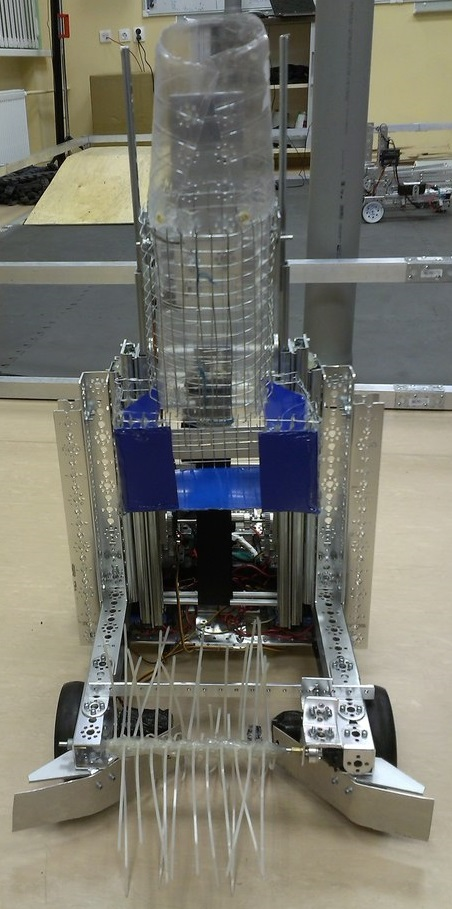
\includegraphics[scale=0.3]{days/17.11.14/images/01}}
				\caption{Ковш в вертикальном положении}
			\end{minipage}
			\hfill
			\begin{minipage}[h]{0.47\linewidth}
				\center{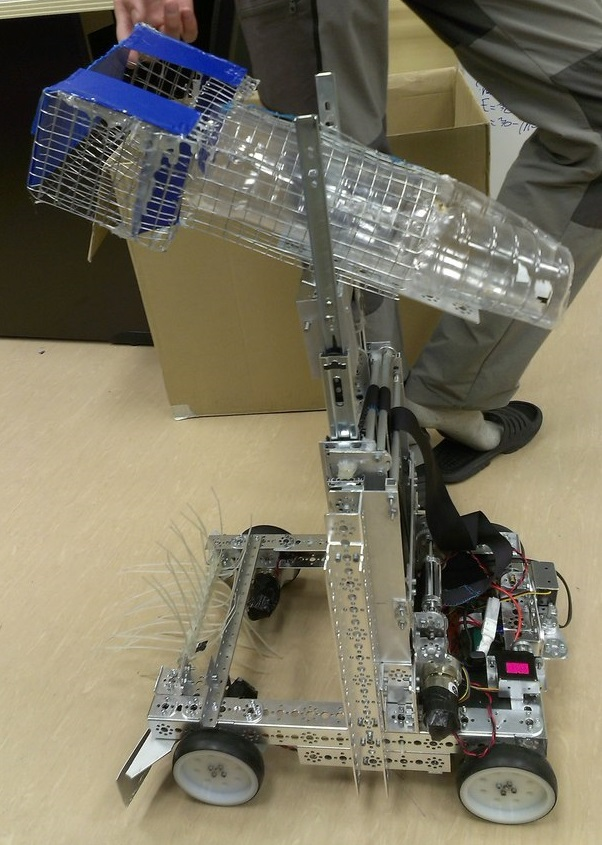
\includegraphics[scale=0.3]{days/17.11.14/images/02}}
				\caption{Ковш в опрокинутом положении}
			\end{minipage}
		\end{figure}
		
		
		\item Ковш был протестирован вручную. В опрокинутом положении мячи скатывались назад без проблем. Всего в ковш зараз помещалось 2 больших мяча и 3 маленьких, что было приемлемо, поскольку на каждый имеющийся на поле большой мяч приходится в среднем 3 маленьких. Дно ковша, выгнутое внутрь, было очень эффективно, поскольку это не давало мячам выпадать из ковша при несильной тряске, неизбежной при движении робота. В целом, мы были удовлетворены работой ковша.
		
		
	\end{enumerate}
	
	\item Итоги собрания:
	\begin{enumerate}
		\item Конструкция ковша завершена.
		
		\item Предварительные испытания ковша не выявили никаких проблем.
		
	\end{enumerate}
	
	\item Задачи для последующих собраний:
	\begin{enumerate}
		\item Испытать ковш в действии с помощью программы.
		
	\end{enumerate}     
\end{enumerate}
\fillpage

